\documentclass[mathserif]{beamer}

\usepackage{microtype}
\usepackage{xparse}
\usepackage{amsmath}
\usepackage{amssymb}
\usepackage{mathtools}
\usepackage{graphicx}

\frenchspacing

\logo{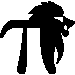
\includegraphics[width=0.07\textwidth]{../Logo}}

\usetheme{Rochester}
\usecolortheme{whale}

\setbeamertemplate{frametitle continuation}[from second][\hfill\insertcontinuationtext]

% Table of contents at start of each section
\AtBeginSection[] {%
	\begin{frame}
		\frametitle{Table of Contents}
		\tableofcontents[currentsection]
	\end{frame}
}

% Environments for math
\newenvironment{compactmath}[1][\normalsize]%
	{\begin{minipage}{\textwidth}\vspace{-0.5\baselineskip}#1\begin{equation*}}
	{\end{equation*}\end{minipage}}

\newenvironment{sizedmath}[1]%
	{\begingroup#1\begin{equation*}}
	{\end{equation*}\endgroup}

% Environments for consistent frame use
\newenvironment{namedframe}[1]%
	{\begin{frame}\frametitle{#1}\framesubtitle{\secname}}
	{\end{frame}}

\newenvironment{namedbreakframe}[1]%
	{\begin{frame}[allowframebreaks]\frametitle{#1}\framesubtitle{\secname}}
	{\end{frame}}

% Frames for emphasis
\newcommand{\sectionstart}[2]{\begin{frame}\frametitle{#1}\centering\Huge\secname\\\Large#2\end{frame}}
\newcommand{\bigframe}[1]{\begin{namedframe}{#1}\Huge\centering#1\end{namedframe}}

% Spacing commands
\newcommand{\sep}{\\\pause\vspace{1ex}}
\newcommand{\varsep}[1]{\\\pause\vspace{#1}}

\newcommand{\vertspace}{\\\vspace{1ex}}
\newcommand{\varvertspace}[1]{\\\vspace{#1}}

% Text formatting
\DeclareTextFontCommand{\emph}{\bfseries}

% Macros for math
\newcommand{\such}{\ |\ }
\DeclarePairedDelimiter{\ceil}{\lceil}{\rceil}
\DeclarePairedDelimiter{\floor}{\lfloor}{\rfloor}


\usepackage{adjustbox}
\usepackage{wrapfig}
\usepackage{textpos}
\usepackage{tikz}
\usetikzlibrary{angles,quotes}

\title{Euclid Preparation 3}
\subtitle{Circle Geometry}
\author{Vincent Macri}
\institute{William Lyon Mackenzie C.I. Math Club}
\date{\copyright{} Caroline Liu, Vincent Macri, and Samantha Unger, 2018}

\includeonly{CrossedChordTheorem}

\begin{document}
	\frame{\titlepage}
	\section{Star Trek Theorem}
		\subsection{Theorem}
\begin{namedframe}{Theorem}
	\vspace{-2ex}
	\begin{theorem}[``Star Trek'' Theorem]
		The central angle \alert{subtended} by any arc is twice any of the inscribed angles on that arc.

		This means that in the diagram, $\angle AOB = 2 \angle ACB$.
	\end{theorem}
	\pause
	\centering
	\begin{columns}
		\begin{column}{0.5\textwidth}
			\centering
			\begin{tikzpicture}[scale=0.4]
				\coordinate [label=left:$O$](O) at (0,0);
				\coordinate [label=below left:$A$](A) at (-3,-4);
				\coordinate [label=below right:$B$](B) at (4,-3);
				\coordinate [label=above left:$C$](C) at (-1,4.89897948557);
				\coordinate [label=below:$L$](L) at (0.5,-2.44948974278);

				\draw (O) circle (5);
				\draw (A) -- (O) -- (B) -- (C) -- cycle;
				\draw [dashed] (C) -- (L);

				\only<6>{\pic [draw, "$\alpha$", angle eccentricity=1.25, angle radius=7mm] {angle = O--A--C};}
				\only<6>{\pic [draw, "$\alpha$", angle eccentricity=1.25, angle radius=7mm] {angle = A--C--O};}

				\only<7>{\pic [draw, "$\beta$", angle eccentricity=1.25, angle radius=1cm] {angle = O--C--B};}
				\only<7>{\pic [draw, "$\beta$", angle eccentricity=1.25, angle radius=1cm] {angle = C--B--O};}
			\end{tikzpicture}
		\end{column}
		\begin{column}{0.5\textwidth}
			Here, $\angle AOB$ is \alert{subtended} by the \alert{minor arc} from $A$ to $B$.
			\sep
			A \alert{minor arc} is the smaller of the two arcs that can be formed by two points on a circle.
			\sep
			Also, note that $\triangle OAC$ and $\triangle OBC$ are isosceles.
			\pause
			This is because $OA$, $OB$, and $OC$ are all radii.
			\pause
			So, $\angle OAC = \angle OCA$ \pause and $\angle OCB = \angle OBC$.
		\end{column}
	\end{columns}
\end{namedframe}
\subsubsection{Proof}
\begin{namedframe}{Proof of the Star Trek Theorem}
	\footnotesize
	\begin{proof}[Proof that $\angle AOB = 2 \angle ACB$]
		\begin{wrapfigure}[0]{r}{0pt}
			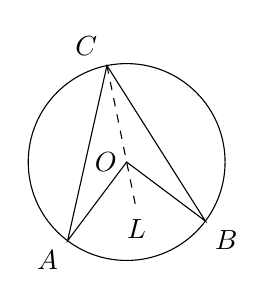
\begin{tikzpicture}[scale=0.25]
				\coordinate [label=left:$O$](O) at (0,0);
				\coordinate [label=below left:$A$](A) at (-3,-4);
				\coordinate [label=below right:$B$](B) at (4,-3);
				\coordinate [label=above left:$C$](C) at (-1,4.89897948557);
				\coordinate [label=below:$L$](L) at (0.5,-2.44948974278);

				\draw (O) circle (5);
				\draw (A) -- (O) -- (B) -- (C) -- cycle;
				\draw [dashed] (C) -- (L);
			\end{tikzpicture}
		\end{wrapfigure}
		We know that $\angle OAC = \angle OCA$.
		\pause
		So: $2\angle OCA + \angle AOC = \SI{180}{\degree}$.
		\sep
		And we know that $\angle AOC + \angle AOL = \SI{180}{\degree}$.
		\pause
		\begin{align*}
			2\angle OCA + \angle AOC &= \angle AOC + \angle AOL\\
			\angle OCA &= \frac{1}{2}\angle AOL
		\end{align*}
		\pause
		And similarly for $\triangle OBC$: $\angle OCB = \frac{1}{2} \angle BOL$.
		\pause
		\begin{align*}
			\uncover<+->{\angle ACB &= \angle OCA + \angle OCB\\}
			\uncover<+->{\angle ACB &= \frac{1}{2}\angle AOL + \frac{1}{2}\angle BOL\\}
			\uncover<+->{\angle ACB &= \frac{1}{2}(\angle AOL + \frac{1}{2}\angle BOL)\\}
			\uncover<+->{2\angle ABC &= \angle AOB}
		\end{align*}
		\uncover<+->{\qedhere}
	\end{proof}
\end{namedframe}

		\subsection{Extensions}
			\bigframe{Extending}
			\subsubsection{Extension 1}
\begin{namedframe}{Diameters and right angles}
	\begin{example}
		Show that if the chord $AB$ is a diameter then $\angle ACB = \SI{90}{\degree}$.

		In other words, show that the angle subtended by a diameter is a right angle.
	\end{example}
	\centering
	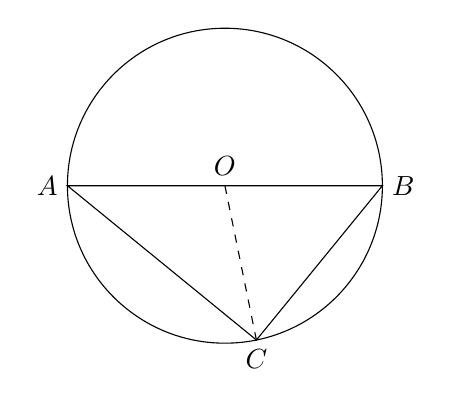
\begin{tikzpicture}[scale=0.4]
		\coordinate [label=above:$O$](O) at (0,0);
		\coordinate [label=left:$A$](A) at (-5,0);
		\coordinate [label=right:$B$](B) at (5,0);
		\coordinate [label=below:$C$](C) at (1,-4.89897948557);

		\draw (O) circle (5);
		\draw (A) -- (O) -- (B) -- (C) -- cycle;
		\draw [dashed] (O) -- (C);
	\end{tikzpicture}
\end{namedframe}
\begin{namedframe}{Proof}
	\footnotesize
	\begin{proof}[Proof that $\angle ACB = \SI{90}{\degree}$.]
		\begin{wrapfigure}[7]{r}{0pt}
			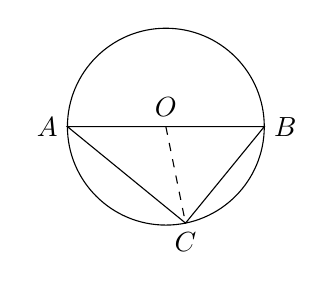
\begin{tikzpicture}[scale=0.25]
				\coordinate [label=above:$O$](O) at (0,0);
				\coordinate [label=left:$A$](A) at (-5,0);
				\coordinate [label=right:$B$](B) at (5,0);
				\coordinate [label=below:$C$](C) at (1,-4.89897948557);

				\draw (O) circle (5);
				\draw (A) -- (O) -- (B) -- (C) -- cycle;
				\draw [dashed] (O) -- (C);
			\end{tikzpicture}
		\end{wrapfigure}
		We know that $\angle ACO = \angle CAO$.
		So:
		\begin{equation}\label{eq:ex1:1}
			2\angle ACO + \angle AOC = \SI{180}{\degree}
		\end{equation}
		\pause
		Similarly:
		\begin{equation}\label{eq:ex1:2}
			2\angle BCO + \angle BOC = \SI{180}{\degree}
		\end{equation}
		\pause
		We also know that $\angle AOC = \SI{180}{\degree} - \angle BOC$.
		\sep[0pt]
		We substitute this into \eqref{eq:ex1:1} to get $2\angle ACO = \angle BOC$.
		\sep[0pt]
		We substitute this into \eqref{eq:ex1:2} to get:
		\begin{align*}
			2\angle BCO + 2\angle ACO &= \SI{180}{\degree}\\
			\angle BCO + \angle ACO &= \SI{90}{\degree}
		\end{align*}
		\pause
		Since $\angle BCO + \angle ACO = \angle ACB$, we arrive at:
		\pause
		\[\angle ACB = \SI{90}{\degree} \qedhere\]
	\end{proof}
\end{namedframe}

			\subsubsection{Extension 2}
\begin{namedframe}{On the major arc}
	\begin{example}
		Show that the Star Trek theorem is still true if $\angle AOB > \SI{180}{\degree}$.
		\vertspace
		That is, show that $\angle AOB = 2\angle ACB$ is true in this diagram.
	\end{example}
	\centering
	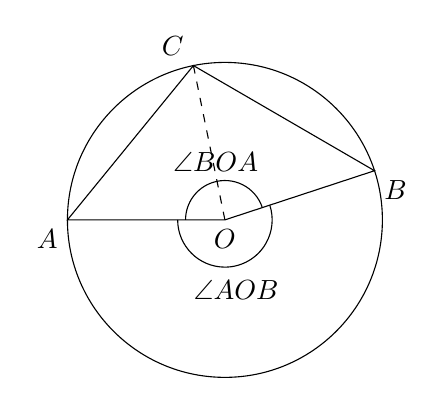
\begin{tikzpicture}[scale=0.4]
		\coordinate [label=below:$O$](O) at (0,0);
		\coordinate [label=below left:$A$](A) at (-5,0);
		\coordinate [label=below right:$B$](B) at (4.75,1.5612494996);
		\coordinate [label=above left:$C$](C) at (-1,4.89897948557);

		\draw (O) circle (5);
		\draw (A) -- (O) -- (B) -- (C) -- cycle;
		\draw [dashed] (O) -- (C);

		\pic [draw, "$\angle BOA$", angle eccentricity=1.5] {angle = B--O--A};
		\pic [draw, "$\angle AOB$", angle eccentricity=1.5, angle radius=6mm] {angle = A--O--B};
	\end{tikzpicture}
\end{namedframe}
\begin{namedframe}{Extension 2 proof}
	\footnotesize
	\begin{proof}[Proof that $\angle AOB = 2\angle ACB $.]
		\vspace{-2ex}
		\begin{wrapfigure}[0]{r}{0pt}
			\scriptsize
			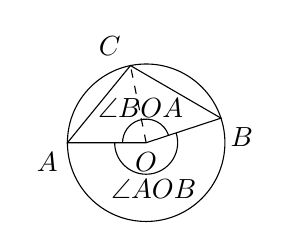
\begin{tikzpicture}[scale=0.2]
				\coordinate [label=below:$O$](O) at (0,0);
				\coordinate [label=below left:$A$](A) at (-5,0);
				\coordinate [label=below right:$B$](B) at (4.75,1.5612494996);
				\coordinate [label=above left:$C$](C) at (-1,4.89897948557);

				\draw (O) circle (5);
				\draw (A) -- (O) -- (B) -- (C) -- cycle;
				\draw [dashed] (O) -- (C);

				\pic [draw, "$\angle BOA$", angle eccentricity=1.5, angle radius=3mm] {angle = B--O--A};
				\pic [draw, "$\angle AOB$", angle eccentricity=1.5, angle radius=4mm] {angle = A--O--B};
			\end{tikzpicture}
		\end{wrapfigure}
		\[2\angle ACO + \angle AOC = \SI{180}{\degree}\]
		\[2\angle BCO + \angle BOC = \SI{180}{\degree}\]
		\sep
		We add these two equations to get:
		\sep[0pt]
		\begin{align*}
			2(\angle ACO + \angle BCO) + \angle AOC + \angle BOC &= \SI{360}{\degree}\\
			2(\angle ACO + \angle BCO) &= \SI{360}{\degree} - (\angle AOC + \angle BOC)
		\end{align*}
		\pause
		We know that $\angle AOC + \angle BOC = \angle BOA$, so:
		\[2(\angle ACO + \angle BCO) = \SI{360}{\degree} - \angle BOA\]
		\pause
		We also know that $\angle AOB = \SI{360}{\degree} - \angle BOA$.
		\sep[0pt]
		And $\angle ACB = \angle ACO + \angle BOC$.
		\pause
		\[\therefore 2\angle ACB = \angle AOB \qedhere\]
	\end{proof}
\end{namedframe}

			\subsubsection{Extension 3}
\begin{namedframe}{Intersecting}
	\begin{example}
		Show that the Star Trek theorem is still true if the point $C$ is chosen so that $AB$ and $OB$ intersect.

		Prove that $\angle AOB = 2 \angle ACB$.
	\end{example}
	\centering
	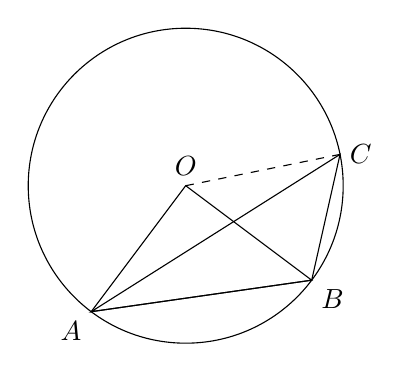
\begin{tikzpicture}[scale=0.4]
		\coordinate [label=above:$O$](O) at (0,0);
		\coordinate [label=below left:$A$](A) at (-3,-4);
		\coordinate [label=below right:$B$](B) at (4,-3);
		\coordinate [label=right:$C$](C) at (4.9,0.994987437107);

		\draw (O) circle (5);
		\draw (A) -- (B) -- (C) -- cycle;
		\draw (A) -- (B) -- (O) -- cycle;
		\draw [dashed] (O) -- (C);
	\end{tikzpicture}
\end{namedframe}
\begin{namedframe}{Extension 3 proof}
	\begin{proof}[Proof that $\angle AOB = 2\angle ACB $.]
		\begin{textblock}{1}(0,0.1)
			\scriptsize
			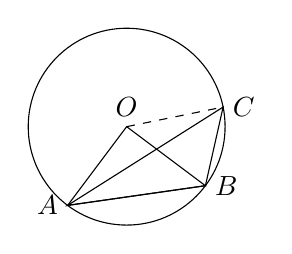
\begin{tikzpicture}[scale=0.25]
				\coordinate [label=above:$O$](O) at (0,0);
				\coordinate [label=left:$A$](A) at (-3,-4);
				\coordinate [label=right:$B$](B) at (4,-3);
				\coordinate [label=right:$C$](C) at (4.9,0.994987437107);

				\draw (O) circle (5);
				\draw (A) -- (B) -- (C) -- cycle;
				\draw (A) -- (B) -- (O) -- cycle;
				\draw [dashed] (O) -- (C);
			\end{tikzpicture}
		\end{textblock}
		\pause
		\begin{equation}\label{eq:ex3:1}
			\angle AOC = \SI{180}{\degree} - 2\angle OCA
		\end{equation}
		\sep[-3ex]
		\begin{equation}\label{eq:ex3:2}
			\angle COB = \SI{180}{\degree} - 2\angle OBC
		\end{equation}
		\sep[-3ex]
		\begin{equation}\label{eq:ex3:3}
			\angle AOB = \angle AOC - \angle COB
		\end{equation}
		\pause
		We can substitute \eqref{eq:ex3:1} and \eqref{eq:ex3:2} into \eqref{eq:ex3:3}:
		\sep[-4ex]
		\begin{align*}
			\angle AOB &= \SI{180}{\degree} - 2\angle OCA - (\SI{180}{\degree} - 2\angle OBC)\\
			\angle AOB &= - 2\angle OCA + 2\angle OBC\\
			\angle AOB &= 2(\angle OBC - \angle OCA)\\
		\end{align*}
		\sep[-4ex]
		We know that know that $\angle ACB = \angle OCB - \angle OCA$.
		\sep[-2ex]
		\[\therefore \angle AOB = 2 \angle ACB \qedhere\]
	\end{proof}
\end{namedframe}

			\subsubsection{Extension 4}
\begin{namedframe}{Cyclic quadrilaterals}
	\transglitter<2>[duration=5]
	\transcover<3>[duration=5]
	\begin{example}
		If $C_1$ and $C_2$ are two points on the circle, one on the minor arc $AB$ and the other on the major arc, prove that $\angle AC_1B + \angle AC_2B = \SI{180}{\degree}$.
		\vertspace
		This is equivalent to proving that the opposite angles of a cyclic quadrilateral are supplementary.
	\end{example}
	\centering
	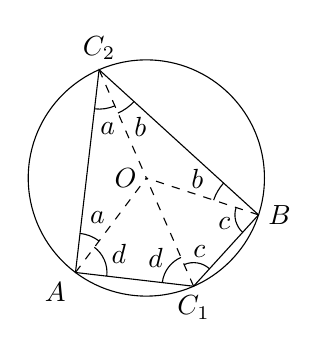
\begin{tikzpicture}[scale=0.3]
		\coordinate [label=left:$O$](O) at (0,0);
		\coordinate [label=below left:$A$](A) at (-3,-4);
		\coordinate [label=right:$B$](B) at (4.75,-1.5612494996);
		\coordinate [label=below:$C_1$](C1) at (2,-4.58257569496);
		\coordinate [label=above:$C_2$](C2) at (-2,4.58257569496);

		\draw (O) circle (5);
		\draw (A) -- (C1) -- (B) -- (C2) -- cycle;
		\draw [dashed] (A) -- (O);
		\draw [dashed] (B) -- (O);
		\draw [dashed] (C1) -- (O);
		\draw [dashed] (C2) -- (O);

		\uncover<3->{\pic [draw, "$a$", angle eccentricity=1.5, angle radius=5mm] {angle = O--A--C2};}
		\uncover<3->{\pic [draw, "$a$", angle eccentricity=1.5, angle radius=5mm] {angle = A--C2--O};}

		\uncover<3->{\pic [draw, "$b$", angle eccentricity=1.5, angle radius=6mm] {angle = C2--B--O};}
		\uncover<3->{\pic [draw, "$b$", angle eccentricity=1.5, angle radius=6mm] {angle = O--C2--B};}

		\uncover<3->{\pic [draw, "$c$", angle eccentricity=1.5, angle radius=3mm] {angle = O--B--C1};}
		\uncover<3->{\pic [draw, "$c$", angle eccentricity=1.5, angle radius=3mm] {angle = B--C1--O};}

		\uncover<3->{\pic [draw, "$d$", angle eccentricity=1.5, angle radius=4mm] {angle = C1--A--O};}
		\uncover<3->{\pic [draw, "$d$", angle eccentricity=1.5, angle radius=4mm] {angle = O--C1--A};}
	\end{tikzpicture}
	\hspace{1cm}
	\uncover<2-2>{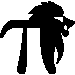
\includegraphics[height=20ex]{../Logo}}
\end{namedframe}
\begin{namedframe}{Extension 4 proof}
	\begin{proof}[Proof that opposite angles of a cycle quadrilateral are supplementary.]
		\begin{wrapfigure}{l}{0pt}
			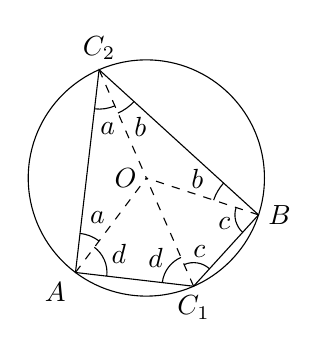
\begin{tikzpicture}[scale=0.3]
				\coordinate [label=left:$O$](O) at (0,0);
				\coordinate [label=below left:$A$](A) at (-3,-4);
				\coordinate [label=right:$B$](B) at (4.75,-1.5612494996);
				\coordinate [label=below:$C_1$](C1) at (2,-4.58257569496);
				\coordinate [label=above:$C_2$](C2) at (-2,4.58257569496);

				\draw (O) circle (5);
				\draw (A) -- (C1) -- (B) -- (C2) -- cycle;
				\draw [dashed] (A) -- (O);
				\draw [dashed] (B) -- (O);
				\draw [dashed] (C1) -- (O);
				\draw [dashed] (C2) -- (O);

				\pic [draw, "$a$", angle eccentricity=1.5, angle radius=5mm] {angle = O--A--C2};
				\pic [draw, "$a$", angle eccentricity=1.5, angle radius=5mm] {angle = A--C2--O};

				\pic [draw, "$b$", angle eccentricity=1.5, angle radius=6mm] {angle = C2--B--O};
				\pic [draw, "$b$", angle eccentricity=1.5, angle radius=6mm] {angle = O--C2--B};

				\pic [draw, "$c$", angle eccentricity=1.5, angle radius=3mm] {angle = O--B--C1};
				\pic [draw, "$c$", angle eccentricity=1.5, angle radius=3mm] {angle = B--C1--O};

				\pic [draw, "$d$", angle eccentricity=1.5, angle radius=4mm] {angle = C1--A--O};
				\pic [draw, "$d$", angle eccentricity=1.5, angle radius=4mm] {angle = O--C1--A};
			\end{tikzpicture}
		\end{wrapfigure}
		\pause
		The sum of the interior angles of a quadrilateral equals \pause $\SI{360}{\degree}$.
		\sep
		So:
		\begin{align*}
			\uncover<+->{a + b + c + d + a + b + c + d &= \SI{360}{\degree}\\}
			\uncover<+->{2(a + b + c + d) &= \SI{360}{\degree}\\}
			\uncover<+->{a + b + c + d &= \SI{180}{\degree}}
		\end{align*}
		\uncover<6->{\qedhere}
	\end{proof}
\end{namedframe}

			\subsubsection{Extension 5}
\begin{namedframe}{Angle subtended by the same chord}
	\begin{example}
		Show that if $C_1$ and $C_2$ are two different choices for the position of the point $C$ along the same arc $AB$ then $\angle AC_1B = \angle AC_2B$.
		\vertspace
		This is equivalent to saying that angles subtended by the same arc are equal.
	\end{example}
	\pause
	\centering
	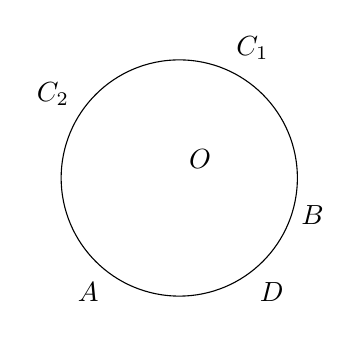
\begin{tikzpicture}[scale=0.3]
		\coordinate [label=above right:$O$](O) at (0,0);
		\coordinate [label=below left:$A$](A) at (-3,-4);
		\coordinate [label=right:$B$](B) at (4.75,-1.5612494996);
		\coordinate [label=above right:$C_1$](C1) at (2,4.58257569496);
		\coordinate [label=above left:$C_2$](C2) at (-4.25,2.63391343821);
		\coordinate [label=below right:$D$](D) at (3,-4);

		\draw (O) circle (5);
	\end{tikzpicture}
	\pause
	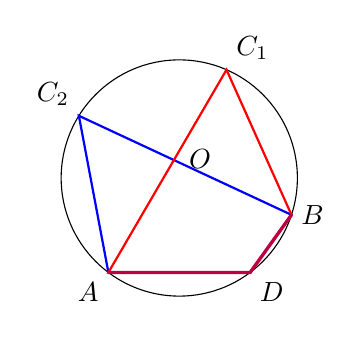
\begin{tikzpicture}[scale=0.3]
		\coordinate [label=above right:$O$](O) at (0,0);
		\coordinate [label=below left:$A$](A) at (-3,-4);
		\coordinate [label=right:$B$](B) at (4.75,-1.5612494996);
		\coordinate [label=above right:$C_1$](C1) at (2,4.58257569496);
		\coordinate [label=above left:$C_2$](C2) at (-4.25,2.63391343821);
		\coordinate [label=below right:$D$](D) at (3,-4);

		\draw (O) circle (5);
		\draw [blue,thick] (A) -- (C2) -- (B) -- (D) -- cycle;
		\draw [red,thick] (A) -- (C1) -- (B) -- (D) -- cycle;
		\draw [purple,very thick] (A) -- (D) -- (B);
	\end{tikzpicture}
\end{namedframe}
\begin{namedframe}{Extension 5 proof}
	\begin{proof}[Proof that $\angle AC_1B = \angle AC_2B$.]
		\begin{wrapfigure}{l}{0pt}
			\scriptsize
			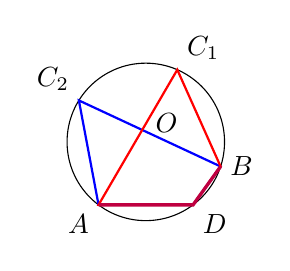
\begin{tikzpicture}[scale=0.2]
				\coordinate [label=above right:$O$](O) at (0,0);
				\coordinate [label=below left:$A$](A) at (-3,-4);
				\coordinate [label=right:$B$](B) at (4.75,-1.5612494996);
				\coordinate [label=above right:$C_1$](C1) at (2,4.58257569496);
				\coordinate [label=above left:$C_2$](C2) at (-4.25,2.63391343821);
				\coordinate [label=below right:$D$](D) at (3,-4);

				\draw (O) circle (5);
				\draw [blue,thick] (A) -- (C2) -- (B) -- (D) -- cycle;
				\draw [red,thick] (A) -- (C1) -- (B) -- (D) -- cycle;
				\draw [purple,very thick] (A) -- (D) -- (B);
			\end{tikzpicture}
		\end{wrapfigure}
		Using extension 4, we know that:
		\pause
		\[\angle AC_1B + \angle ADB = \SI{180}{\degree}\]
		\pause
		\[\angle AC_2B + \angle ADB = \SI{180}{\degree}\]
		\sep[5ex]
		So:
		\pause
		\begin{align*}
			\angle AC_1B + \angle ADB &= \angle AC_2B + \angle ADB\\
			\angle AC_1B &= \angle AC_2B \qedhere
		\end{align*}
	\end{proof}
\end{namedframe}

	\section{Crossed Chord Theorem}
		\subsection{Theorem}
\begin{namedframe}{Theorem}
	\begin{theorem}[``Crossed Chord'' Theorem]
		If two chords $AB$ and $CD$ of a circle intersect at point $P$, then $(PA)(PB) = (PC)(PD)$.
	\end{theorem}
	\vspace{-2ex}
	\begin{center}
		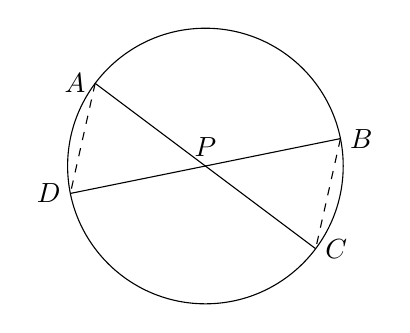
\begin{tikzpicture}[scale=0.35]
			\coordinate [label=above:$P$](P) at (0,0);
			\coordinate [label=left:$A$](A) at (-4,3);
			\coordinate [label=right:$B$](B) at (4.9,0.994987437107);
			\coordinate [label=right:$C$](C) at (4,-3);
			\coordinate [label=left:$D$](D) at (-4.9,-0.994987437107);

			\draw (P) circle (5);
			\draw (A) -- (P) -- (B);
			\draw (D) -- (P) -- (C);
			\draw [dashed] (B) -- (C);
			\draw [dashed] (A) -- (D);
		\end{tikzpicture}
	\end{center}
	\vsep[-2ex]
	This is proved using similar triangles and the fifth extension we developed for the Star Trek theorem.
	Try to prove it yourself!
\end{namedframe}

\end{document}
